\documentclass[twocolumn,english]{article}
\renewcommand{\familydefault}{\sfdefault}
\usepackage[T1]{fontenc}
\usepackage[latin9]{inputenc}
\usepackage[landscape]{geometry}
\geometry{verbose,tmargin=0.5in,bmargin=0.75in,lmargin=0.5in,rmargin=0.5in}
\setlength{\parskip}{0bp}
\setlength{\parindent}{0pt}
\usepackage{float}
\usepackage{booktabs}
\usepackage{algorithm2e}
\usepackage{amsmath}
\usepackage{amssymb}
\usepackage{graphicx}
\PassOptionsToPackage{normalem}{ulem}
\usepackage{ulem}

\makeatletter

\providecommand{\tabularnewline}{\\}

\RequirePackage{fix-cm}
\RequirePackage{fixltx2e}



\usepackage{enumitem}
\usepackage{amsthm}
\PassOptionsToPackage{normalem}{ulem}




\providecommand{\tabularnewline}{\\}

 % used for custom paragraph shapes
 \IfFileExists{candleshape.def}{%
  \input{candleshape.def}}{}
 \IfFileExists{dropshape.def}{%
  \input{dropshape.def}}{}
 \IfFileExists{TeXshape.def}{%
  \input{TeXshape.def}}{}
 \IfFileExists{triangleshapes.def}{%
  \input{triangleshapes.def}}{}

\newlength{\lyxlabelwidth}      % auxiliary length 
\numberwithin{equation}{section}
\numberwithin{figure}{section}
\numberwithin{table}{section}




\usepackage{array}
\usepackage{multirow}





\providecommand{\tabularnewline}{\\}

\setlength{\columnsep}{0.25in}
\usepackage{xcolor}
\usepackage{textcomp}
\usepackage{listings}
\lstset{
  tabsize=2,
  basicstyle=\small\ttfamily,
}



\usepackage{babel}
\usepackage{listings}
\renewcommand{\lstlistingname}{Listing}


\usepackage{titlesec}
\titleformat*{\section}{\color{blue!60!green!40!black} \vspace{8pt}\titlerule\vspace{4pt}\Large\bfseries\sffamily}
\titleformat*{\subsection}{\color{blue!60!green} \vspace{2pt}\large\bfseries\sffamily}



\usepackage{enumitem}
\setlist{itemsep=0pt}


\let\emph\relax
\DeclareTextFontCommand{\emph}{\bfseries}



\usepackage{babel}
\usepackage{listings}
\renewcommand{\lstlistingname}{Listing}

\makeatother

\usepackage{babel}
\usepackage{listings}
\renewcommand{\lstlistingname}{Listing}

\begin{document}

\title{\vspace{-4ex}
Revision Notes for CO202 Algorithms II\vspace{-4ex}
}


\date{Spring 2018\vspace{-2ex}
}

\maketitle
 


\section{Order of Growth}
\begin{itemize}
\item \emph{Asymptotic bound}: $f\left(n\right)$ is order $\Theta\left(g\left(n\right)\right)$
if there is $c_{1},c_{2},n_{0}>0$ such that $0\leq c_{1}g\left(n\right)\leq f\left(n\right)\leq c_{2}g\left(n\right)$
for all $n\geq n_{0}$. 
\item \emph{Asymptotic upper bound}: $f\left(n\right)$ is order $O\left(g\left(n\right)\right)$
if there is $c,n_{0}>0$ such that $0\leq f\left(n\right)\leq cg\left(n\right)$
for all $n\geq n_{0}$. 
\item \emph{Asymptotic lower bound}: $f\left(n\right)$ is order $\Omega\left(g\left(n\right)\right)$
if there is $c,n_{0}>0$ such that $0\leq cg\left(n\right)\leq f\left(n\right)$
for all $n\geq n_{0}$. 
\end{itemize}
\emph{Note}: \uline{not} average / best / worst case.


\section{Divide and Conquer}
\begin{enumerate}
\item \emph{Divide} the problem into smaller sub-problems. 
\item \emph{Conquer} sub-problems by solving recursively (recursive case).
If size is small enough, can be solved trivially (base case). 
\item \emph{Combine} solutions to sub-problems into final solution. 
\end{enumerate}

\subsubsection*{Recurrences}

Equations that describe functions in terms of its value on smaller
inputs. Assuming: 
\begin{enumerate}
\item Trivial problems $n\leq c$ solved in constant time. 
\item Division yields $a$ sub-problems, each of size $1/b$. 
\item Divide takes time $D\left(n\right)$ and combine $C\left(n\right)$. 
\end{enumerate}
\[
T\left(n\right)=\begin{cases}
\Theta\left(1\right) & n\leq c\\
aT\left(\frac{n}{b}\right)+D\left(n\right)+C\left(n\right) & \text{otherwise}
\end{cases}
\]



\paragraph{Solving Recurrences}
\begin{enumerate}
\item \emph{Substitution}: guess and use induction to prove. (Guess $O\left(f\left(n\right)\right)$
and then prove $T\left(n\right)\leq cf\left(n\right)$). For the induction:

\begin{enumerate}
\item \emph{Use constants} wherever necessary.
\item \emph{Use strong induction}. Try assuming it holds for $n/b$. 
\item Choose \emph{any valid base case}.
\item If stuck, \emph{strengthen inductive hypothesis}. Subtracting lower
order terms can help (e.g. prove $T\left(n\right)\leq cn^{2}-kn$
instead of $T\left(n\right)\leq cn^{2}$). 
\end{enumerate}
\item \emph{Recursion Tree}: Convert recurrence into a tree whose nodes
are costs at different levels. 

\begin{enumerate}
\item Substitute directly into the tree.
\item Remember that $k^{\log_{c}n}=n^{\log_{c}k}$ and $\sum_{k=0}^{n}c^{k}=\frac{1-c^{n}}{1-c}$.
\end{enumerate}
\item \emph{Simple Master Theorem}: For $T\left(n\right)=aT\left(n/b\right)+\Theta(n^{d})$: 

\begin{enumerate}
\item If $d<\log_{b}a$, then $T\left(n\right)=\Theta\left(n^{\log_{b}a}\right)$. 
\item If $d=\log_{b}a$, then $T\left(n\right)=\Theta\left(n^{d}\lg n\right)$. 
\item If $d>\log_{b}a$, then $T\left(n\right)=\Theta\left(n^{d}\right)$. 
\end{enumerate}
\item \emph{Generic Master Theorem}: For $T\left(n\right)=aT\left(n/b\right)+f\left(n\right)$,
if for some constant $\epsilon>0$:

\begin{enumerate}
\item $f\left(n\right)=O\left(n^{\log_{b}a-\epsilon}\right)$, then $T\left(n\right)=\Theta\left(n^{\log_{b}a}\right)$. 
\item $f\left(n\right)=\Theta\left(n^{\log_{b}a}\right)$, then $T\left(n\right)=\Theta\left(n^{\log_{b}a}\lg n\right)$. 
\item $f\left(n\right)=\Omega\left(n^{\log_{b}a+\epsilon}\right)$, then
$T\left(n\right)=\Theta\left(f\left(n\right)\right)$.\medskip{}
\\
For (c) the \emph{regularity condition} must hold: $af\left(n/b\right)\leq cf$$\left(n\right)$
for some constant $c<1$ and all sufficielntly large $n$.
\end{enumerate}
\end{enumerate}

\subsubsection*{Example: Merge Sort}

\begin{lstlisting}[language=Python,basicstyle={\footnotesize\ttfamily},tabsize=4,frame=single]
MERGE-SORT(A, p, r):
	if p < r:                     # more than one item?
		q = floor((p + r)/2)      # divide array
		MERGE-SORT(A, p, q)       # conquer 1st subarray
		MERGE-SORT(A, q + 1, r)   # conquer 2nd subarray
		MERGE(A, p, q, r)         # combine subarrays
\end{lstlisting}


The \emph{combine} step:

\begin{lstlisting}[language=Python,basicstyle={\footnotesize\ttfamily},tabsize=4,frame=single]
MERGE(A, p, q, r):
n1 = q - p + 1                    # length of 1st subarray
n2 = r - q                        # length of 2nd subarray
let L[1..n1 + 1] and R[1..n2 + 1] be new arrays
for i = 1 to n1:
	L[i] = A[p + i - 1]           # copy values to 1st array
for j = 1 to n2:
	R[j] = A[q + j]               # copy values to 2nd array
L[n1 + 1] = inf                   # set sentinel
R[n2 + 1] = inf                   # set sentinel
i = 1
j = 1
for k = p to r:                   # merge subarrays
	if L[i] <= R[j]:
		A[k] = L[i]
		i = i + 1
	else:
		A[k] = R[j]
		j = j + 1
\end{lstlisting}


Takes time: 
\[
T\left(n\right)=\begin{cases}
\Theta\left(1\right) & n=1\\
2T\left(\left\lfloor \frac{n}{2}\right\rfloor \right)+\Theta\left(n\right) & n>1
\end{cases}=\Theta\left(n\lg n\right)
\]



\section{Dynamic Programming}
\begin{itemize}
\item Combines solutions to overlapping sub-problems. 
\item Saves its answer in a table to avoid re-computation. 
\end{itemize}

\paragraph{Requirements}
\begin{itemize}
\item \emph{Optimal substructure}: Optimal solution contains optimal solution
to sub-problems. 
\item \emph{Overlapping sub-problems}: Solution combines solutions to overlapping
sub-problems. 
\end{itemize}

\paragraph{Developing a DP Algorithm}
\begin{enumerate}
\item Characterise the structure of an optimal solution. 
\item Recursively define the value of an optimal solution: \emph{test your
definition very carefully}.
\item Compute the value of an optimal solution, in a bottom-up fashion. 
\item Construct an optimal solution from computed information. 
\end{enumerate}

\paragraph{Top-Down with Memoisation vs. Bottom-Up}
\begin{itemize}
\item Bottom-up is more efficient by a constant factor because there is
no overhead for recursive calls. 
\item Bottom-up may benefit from optimal memory access. 
\item Top-down can avoid computing solutions of sub-problems that are not
required. 
\item Top-down is `more natural'. 
\end{itemize}

\paragraph{Recording the Solution}

Keep an additional array to record which sub-problem was used.


\paragraph{Example 1: Rod Cutting}
\begin{itemize}
\item A rod of length $i$ is worth $p_{i}$. 
\item The maximum revenue, $r_{n}=\max_{1\leq i\leq n}\left(p_{i}+r_{n-i}\right)$. 
\end{itemize}
\begin{lstlisting}[language=Python,basicstyle={\footnotesize\ttfamily},tabsize=4,frame=single]
#### Top-Down with Memoisation
MEMOIZED-CUT-ROD(p, n):
	let r[0..n] be a new array
	for i = 0 to n:
		r[i] = -inf
	return MEMOIZED-CUT-ROD-AUX(p, n, r)

MEMOIZED-CUT-ROD-AUX(n, p, r):
	if r[n] >= 0
		return r[n]
	if n == 0:
		q = 0
	else:
		q = -inf
		for q = 1 to n
			q = max(q, p[i] + MEMOIZED-CUT-ROD-AUX(p, n - i, r)
	r[n] = q
	return q

#### Bottom-Up
BOTTOM-UP-CUT-ROD(p, n):
	let r[0..n] be a new array
	r[0] = 0
	for j = 1 to n:
		q = -inf
		for i = 1 to j:
			q = max(q, p[i] + r[j - i])
		r[j] = q
	return r[n]
\end{lstlisting}



\paragraph{Example 2: Longest Common Subsequence}


\subparagraph{Step 1: Find optimal structure.}

For $X=\left\langle x_{1},\dots,x_{m}\right\rangle $, $Y=\left\langle y_{1},\dots,y_{n}\right\rangle $
and $Z=\left\langle z_{1},\dots,z_{k}\right\rangle $, where $Z$
is the LCS of $X$ and $Y$: 
\begin{enumerate}
\item If $x_{m}=y_{n}$, then $z_{k}=x_{m}=y_{n}$ and $Z_{k-1}$ is LCS
of $X_{m-1}$ and $Y_{n-1}$. 
\item If $x_{m}\neq y_{n}$, then $z_{k}\neq x_{m}$ implies that $Z$ is
LCS of $X_{m-1}$ and $Y$. 
\item If $x_{m}\neq y_{n}$, then $z_{k}\neq y_{n}$ implies that $Z$ is
LCS of $X$ and $Y_{n-1}$. 
\end{enumerate}

\subparagraph{Step 2: Define recursive solution.}

Where $l\left(i,j\right)$ is the length of an LCS of sequences $X_{i..m}$
and $Y_{j..n}$:

\[
l\left(i,j\right)=\begin{cases}
0 & \text{if \ensuremath{i=m} or \ensuremath{j=n} (base case)}\\
l\left(i-1,j-1\right)+1 & \text{if \ensuremath{i<m}, \ensuremath{j<n} and \ensuremath{x_{i}=y_{j}} (case 1)}\\
\max\begin{cases}
l(i-1,j) & \text{(case 2)}\\
l\left(i,j-1\right) & \text{(case 3)}
\end{cases} & \text{if \ensuremath{i<m}, \ensuremath{j<n} and \ensuremath{x_{i}\neq y_{j}})}
\end{cases}
\]



\subparagraph{Steps 3 and 4: Compute value and construct solution.}


\paragraph{Example 3: Levenshtein Distance}

Where $d\left(i,j\right)$ is the edit distance of sequences~$X_{i..m}$
and $Y_{j..n}$: 
\[
d\left(i,j\right)=\begin{cases}
\max\left(i,j\right) & \text{if \ensuremath{i=0} or \ensuremath{j=0} (base case)}\\
\min\begin{cases}
d\left(i-1,j\right)+1 & \text{(delete)}\\
d\left(i,j-1\right)+1 & \text{(insert)}\\
d(i-1,j-1) & \text{(no-op)}
\end{cases} & \text{if \ensuremath{i<m}, \ensuremath{j<n} and \ensuremath{x_{i}=y_{j}}}\\
\min\begin{cases}
d\left(i-1,j\right)+1 & \text{(delete)}\\
d\left(i,j-1\right)+1 & \text{(insert)}\\
d(i-1,j-1)+1 & \text{(replace)}
\end{cases} & \text{if \ensuremath{i<m}, \ensuremath{j<n} and \ensuremath{x_{i}\neq y_{j}}}
\end{cases}
\]



\section{Greedy Algorithms}
\begin{itemize}
\item Applied to optimisation problems. 
\item When there is a choice, always make the choice that looks best at
the moment (don't look ahead). 
\end{itemize}

\paragraph{Requirements}
\begin{enumerate}
\item \emph{Optimal substructure}: Optimal solution contains optimal solutions
to sub-problems. 
\item \emph{Greedy-choice property}: Globally optimal solution obtained
through locally optimal choices. 
\end{enumerate}

\paragraph{Developing a Greedy Algorithm}
\begin{enumerate}
\item Demonstrate optimal substructure. 
\item Cast the problem as one in which making a choice only leaves one sub-problem
to solve. 
\item Prove the optimality of the solution when making greedy choices. 
\end{enumerate}

\paragraph{Example 1: Activity Selection Problem}

Given a set of proposed activities, $S=\left\{ a_{1},a_{2},\dots,a_{n}\right\} $,
each $a_{i}$ having a start time $s_{i}$ and finish time $f_{i}$,
which all use the same resource, find maximum number of mutually compatible
activities. 
\begin{enumerate}
\item \emph{Greedy choice}: choose the activity $a_{k}$ with earliest finish
time. 
\item Solve the sub-problem with $S_{k}=\left\{ a_{i}\in S\text{ such that }s_{i}\geq f_{k}\right\} $. 
\end{enumerate}
\begin{lstlisting}[language=Python,basicstyle={\footnotesize\ttfamily},tabsize=4,frame=single]
# Assuming activities are ordered by finish time
ACTIVITY-SELECTOR(s, f):
	n = len(s)
	A = [s[0]]
	k = 0
	for m = 1 to n - 1:
		if s[m] >= f[k]:
			A = A + [s[m]]
			k = m
	return A
\end{lstlisting}



\paragraph{Example 2: Fractional Knapsack Problem}

\emph{Greedy choice}: choose item with maximum value per unit weight.


\section{Randomised Algorithms}


\paragraph{Strategies}
\begin{enumerate}
\item Randomise the \emph{input} (e.g. random permutations \textemdash{}
hiring problem). 
\item Randomise the \emph{computation} (e.g. random choices \textemdash{}
quicksort / BST insert). 
\end{enumerate}

\paragraph{Benefits}
\begin{enumerate}
\item Help avoid pathologic inputs. 
\item Yield good expected running time. 
\item Allow dealing with large input domains. 
\end{enumerate}

\paragraph{Example 1: Hiring Problem}

Randomise the input to reduce the chance of worst-case.


\paragraph{Example 2: Quicksort}
\begin{enumerate}
\item \emph{Divide}: partition the array \texttt{A{[}p..r{]}} into \texttt{A{[}p..q-1{]}}
and \texttt{A{[}q+1..r{]}} with all elements less than or equal to
and greater than or equal to \texttt{A{[}q{]}} respectively. 
\item \emph{Conquer}: sort the two subarrays recursively using quicksort. 
\end{enumerate}
Running time depends on whether partitioning is balanced or unbalanced: 
\begin{itemize}
\item \emph{Balanced}: runs asymptotically as fast as merge sort. 
\[
T\left(n\right)=2T\left(n/2\right)+\Theta\left(n\right)=\Theta\left(n\lg n\right)
\]

\item \emph{Unbalanced}: can run asymptotically as fast as insertion sort.
\[
T\left(n\right)=T\left(n-1\right)+T\left(0\right)+\Theta\left(n\right)=\Theta\left(n^{2}\right)
\]

\end{itemize}
Possible solution: 
\begin{itemize}
\item Select pivot using random sampling (or median of 3 randomly selected
samples). 
\end{itemize}

\paragraph{Example 3: Binary Search Trees}
\begin{itemize}
\item \emph{BST property}: For every node $y$ in the left subtree of $x$,
$y.\text{key}\leq x.\text{key}$ and every node $z$ in the right
subtree of $x$, $y.\text{key}\geq z.\text{key}$. 
\item Insert and search have complexity $O\left(h\right)$ where $h$ is
the height of the tree. 
\end{itemize}
Expected height of randomly built BST with $n$ keys is $O\left(\lg n\right)$.
Try to achieve by: 
\begin{itemize}
\item Randomly permute input (if known in advance). 
\item Recursively choose to insert at the root (by using \emph{rotations})
with probability $1/\text{size}$ or as a leaf. 
\end{itemize}
\begin{figure}[H]
\centering{}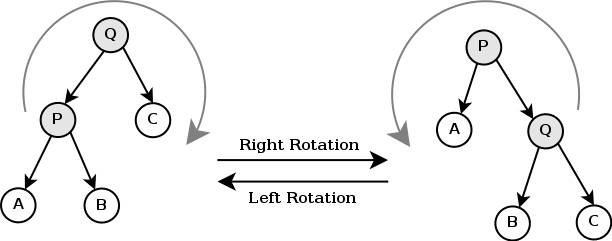
\includegraphics[width=0.5\linewidth]{img/rotate} 
\end{figure}



\paragraph{Example 4: Skip Lists}
\begin{itemize}
\item Maintain a hierarchy of linked sublists. 
\item Good for fast \emph{search of ordered sequence}. 
\end{itemize}
Not feasible to maintain ideal skip-list as we need to reorganise
after each insert. Solution: 
\begin{itemize}
\item An element in layer $i$ appears with some probability in layer $i+1$. 
\end{itemize}

\paragraph{Example 5: Find a Zero Bit}

From an array of 0 and 1 bits. Possible \emph{generate and test} algorithms: 
\begin{itemize}
\item \emph{Las Vegas Algorithm}: choose an index randomly until you find
a 0. 

\begin{itemize}
\item Always correct but unbounded resources. 
\end{itemize}
\item \emph{Monte Carlo Algorithm}: choose up to $k$ random indices attempting
to find a 0. 

\begin{itemize}
\item Not always correct but bounded resources. 
\end{itemize}
\end{itemize}

\section{Visualising Algorithms}

Provide \emph{understanding} and \emph{insights} into characteristics
and support \emph{debugging}.


\subsection{Sorting}


\paragraph{Visualisation Methods}
\begin{itemize}
\item Animations. 
\item Weave visualisations. 
\item Leaning lines. 
\end{itemize}

\subsection{Random Sampling}


\subsubsection*{Uniform Sampling}

\begin{lstlisting}[language=Python,basicstyle={\footnotesize\ttfamily},tabsize=4,frame=single]
UNIFORM-SAMPLE(width, height):
	x = RANDOM-REAL(0, 1) * width
	y = RANDOM-REAL(0, 1) * height
	return (x, y)
\end{lstlisting}



\subsubsection*{Best-Candidate Sampling}

\begin{lstlisting}[language=Python,basicstyle={\footnotesize\ttfamily},tabsize=4,frame=single]
BEST-CANDIDATE-SAMPLE(width, height, samples, n):
	best_candidate = (0, 0)
	best_distance  = 0
	for i = 1 to n:
		c = UNIFORM-SAMPLE(width, height)
		d = DISTANCE(FIND-CLOSEST(samples, c), c)
		if d > best_distance
			best_distance = d
			best_candidate = c
return best_candidate
\end{lstlisting}



\subsubsection*{Poisson-Disc Sampling}
\begin{itemize}
\item Use a grid (each to contain a maximum of one sample) to speed up searches. 
\item Select a first sample randomly and make it \emph{active}. 
\item Choose an \emph{active} sample and generate up $k$ points between
radius $r$ and $2r$ from the sample. 

\begin{itemize}
\item If a point is ever found further than $r$ from all other samples
(check using the grid), choose it and make it \emph{active}. 
\item Otherwise, make this point not \emph{active}. 
\end{itemize}
\end{itemize}

\paragraph{Visualisation Methods}
\begin{itemize}
\item Histograms ($x,y$ coordinates or minimum distances). 
\item Scatter plots. 
\item Voronoi diagrams. 
\end{itemize}

\subsection{Random Shuffling}

Want to find \emph{unbiased} algorithm (every permutation equally
likely).


\subsubsection*{Fisher-Yates Shuffling}

\begin{lstlisting}[language=Python,basicstyle={\footnotesize\ttfamily},tabsize=4,frame=single]
FISHER-YATES-SHUFFLE(A):
for i = n down to 2:
	j = RANDOM(1, i)   # make sure i is included
	SWAP(A[i], A[j])
\end{lstlisting}



\paragraph{Visualisation Methods}
\begin{itemize}
\item Leaning lines. 
\item Swap matrices. 
\end{itemize}

\section{String Matching}

For text $T\left[1..n\right]$, attempt to find a pattern $P\left[1..m\right]$
with $m\leq n$.


\paragraph{Definitions}
\begin{itemize}
\item $P$ occurs in $T$ with \emph{shift} $s$ if $T\left[s+j\right]=P\left[j\right]$
for $1\leq j\leq m$. 
\item $w\sqsubset x$ if $w$ is a prefix of $x$. 
\item $w\sqsupset x$ if $w$ is a suffix of $x$. 
\item The prefix $P\left[1..k\right]$ of a pattern $P\left[1..m\right]$
is denoted $P_{k}$. 
\end{itemize}
If $x$ and $y$ are suffixes of $z$: 
\begin{itemize}
\item If $\left|x\right|\leq\left|y\right|$, then $x$ is a suffix of $y$. 
\item If $\left|x\right|\geq\left|y\right|$, then $y$ is a suffix of $x$. 
\item If $\left|x\right|=\left|y\right|$, then $x=y$. 
\end{itemize}

\subsection{Knuth-Morris-Pratt Matching}
\begin{itemize}
\item \emph{Key Idea}: Go through $T$ character by character, use a prefix
function 
\[
\pi\left[q\right]=\max\left(k\text{ such that }k<q\text{ and }P_{k}\text{ is a suffix of }P_{q}\right)
\]
Example: 
\begin{table}[H]
\centering{}%
\begin{tabular}{cccccccc}
\toprule 
$i$  & 1  & 2  & 3  & 4  & 5  & 6  & 7\tabularnewline
\midrule 
$P\left[i\right]$  & \texttt{a}  & \texttt{b}  & \texttt{a}  & \texttt{b}  & \texttt{a}  & \texttt{c}  & \texttt{a}\tabularnewline
$\pi\left[i\right]$  & 0  & 0  & 1  & 2  & 3  & 0  & 1\tabularnewline
\bottomrule
\end{tabular}
\end{table}

\item \texttt{PREFIX-FUNCTION} takes $O\left(m\right)$ and \texttt{KMP-MATCHER}
$O\left(n\right)$ time. 
\end{itemize}
\begin{figure}[H]
\centering{}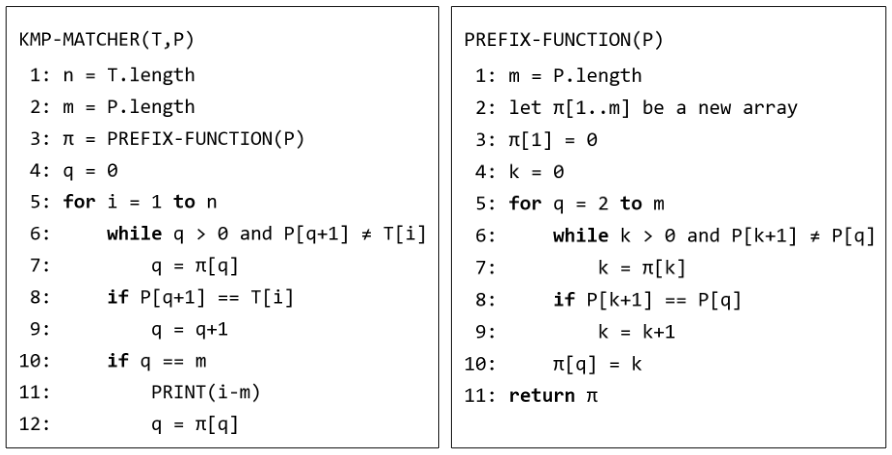
\includegraphics[width=0.8\linewidth]{img/kmp-matching} 
\end{figure}



\subsection{Boyer-Moor Matching}
\begin{itemize}
\item Start matching from the right of $P$. When matching breaks, shift
$P$ as far right as possible, maximising skipped comparisons. 
\item \emph{Bad character rule}: Current character ($\beta$) in $T$ doesn't
match current character in $P$. 

\begin{itemize}
\item If $\beta$ not in $P$, shift $P$ so that it skips $\beta$. 
\item If $\beta$ is in $P$, shift $P$ so it aligns that the right-most
$\beta$ in $P$. 
\begin{table}[H]
\centering{}For $P=\texttt{ababaca}$: %
\begin{tabular}{cccc}
\toprule 
$c$  & \texttt{a}  & \texttt{b}  & \texttt{c}\tabularnewline
\midrule 
$\text{bcr}\left[c\right]$  & \texttt{7}  & 4  & 6\tabularnewline
\bottomrule
\end{tabular}
\end{table}

\end{itemize}
\item \emph{Good suffix rule}: A suffix of $P$ has been matched in $T$
up to a bad character in $T$. 

\begin{itemize}
\item If the match occurs somewhere else in $P$, shift to align it with
the right-most occurrence in $P$. 
\item If the match occurs nowhere else in the pattern, skip the pattern. 
\item If the prefix of $P$ matches the suffix of the match, align the prefix
of $P$ with the suffix of the match. 
\begin{table}[H]
\centering{}%
\begin{tabular}{ccccccccc}
\toprule 
$i$  & 1  & 2  & 3  & 4  & 5  & 6  & 7  & 8\tabularnewline
\midrule 
$P\left[i\right]$  & \texttt{a}  & \texttt{b}  & \texttt{a}  & \texttt{b}  & \texttt{a}  & \texttt{c}  & \texttt{a}  & $\epsilon$\tabularnewline
$\text{gsr}\left[i\right]$  & 6  & 6  & 6  & 6  & 6  & 2  & 1  & $\slash$\tabularnewline
\bottomrule
\end{tabular}
\end{table}



\begin{table}[H]
\centering{}%
\begin{tabular}{ccccccc}
\toprule 
$i$  & 1  & 2  & 3  & 4  & 5  & 6\tabularnewline
\midrule 
$P\left[i\right]$  & \texttt{c}  & \texttt{a}  & \texttt{b}  & \texttt{a}  & \texttt{b}  & $\epsilon$\tabularnewline
$\text{gsr}\left[i\right]$  & 5  & 5  & 2  & 5  & 1  & $\slash$\tabularnewline
\bottomrule
\end{tabular}
\end{table}


\end{itemize}
\item \texttt{BCR-TABLE} and \texttt{GSR-TABLE} take $O\left(m\right)$
and \texttt{BM-MATCHER} $O\left(mn\right)$ time. 
\end{itemize}

\section{Radix Search}

Examine keys one piece at a time, rather than a full comparison.


\paragraph{Digital Search Trees}

Exactly the same as BSTs except left/right branching is not based
on full comparisons, but selected bits of keys.

\begin{figure}[H]
\centering{}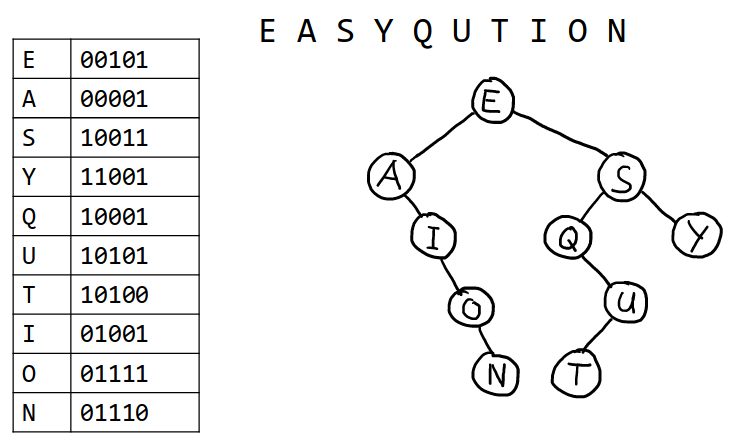
\includegraphics[width=0.625\linewidth]{img/dst} 
\end{figure}

\begin{itemize}
\item Still compares whole keys. 
\item Maximum depth is the maximum key length ($b$). 
\item Keys with similar prefixes degrade performance. 
\end{itemize}

\paragraph{Binary Search Tries}

Keys are only stored at the leaf nodes.

\begin{figure}[H]
\centering{}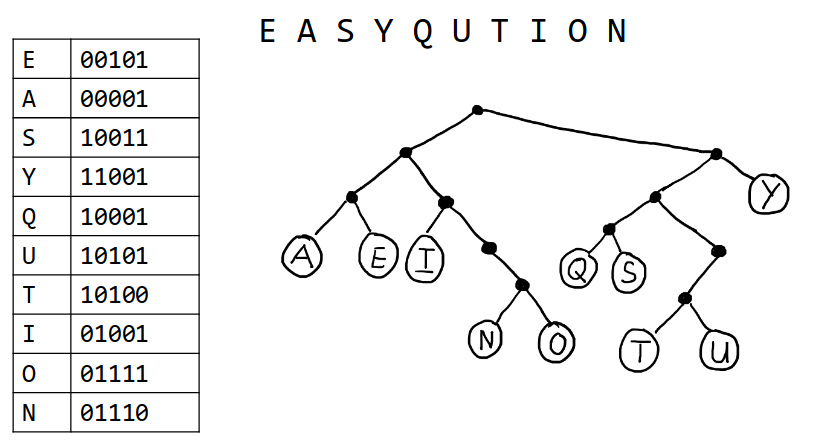
\includegraphics[width=0.75\linewidth]{img/bst} 
\end{figure}

\begin{itemize}
\item Don't compare the full key until a leaf is reached. 
\item For $n$ keys, average search requires $\lg n$ comparisons and $b$
in worst case. 
\item One-way branching creates extra unnecessary nodes in the trie. 
\item Two different types of nodes means implementation is complex. 
\end{itemize}

\paragraph{Patricia Tries}
\begin{itemize}
\item Each node includes the index of the bit to be tested. 
\item Uses pointers up the tree instead of NULLs. 
\item \emph{Search}: Follow pointers until they point at the \emph{same
level} or \emph{up} the trie. Then check this node.
\end{itemize}
\begin{figure}[H]
\centering{}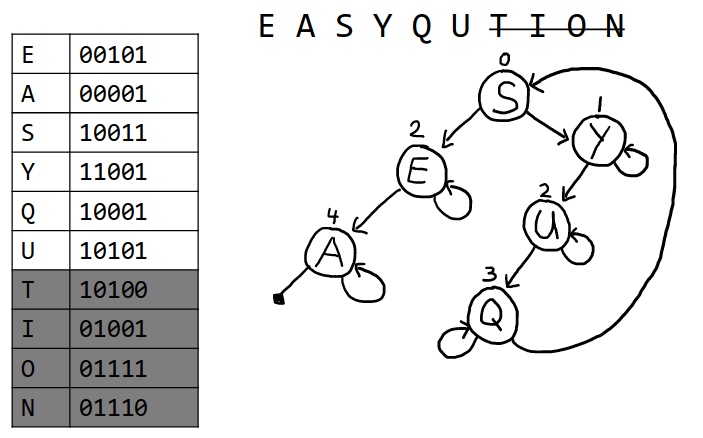
\includegraphics[width=0.5\linewidth]{img/pt} 
\end{figure}

\begin{itemize}
\item Only has $n$ nodes. 
\item Only requires about $\lg n$ bit comparisons. 
\end{itemize}

\paragraph{Multiway Search Tries}

Examine $r$ bits at a time, using nodes with $R=2^{r}$ links.

\begin{figure}[H]
\centering{}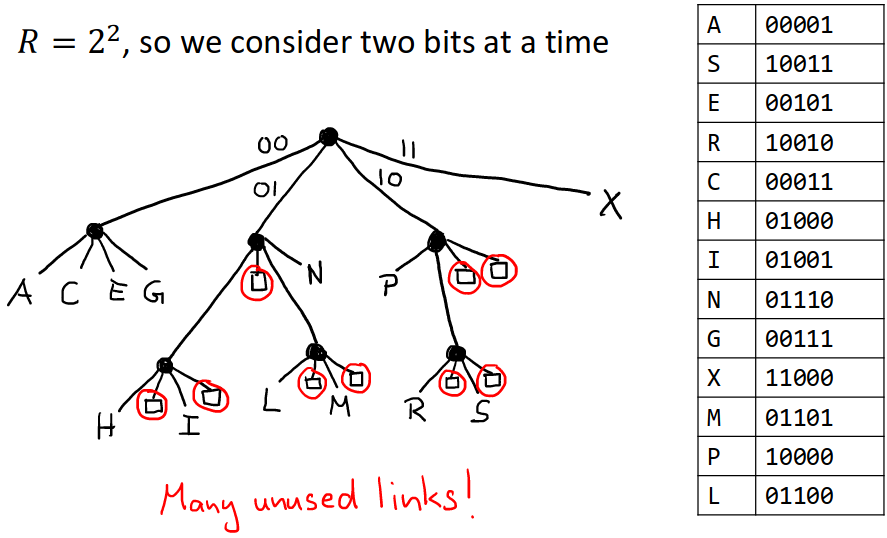
\includegraphics[width=0.75\linewidth]{img/multiwayst} 
\end{figure}

\begin{itemize}
\item Requires $O\left(\log_{R}n\right)$ comparisons. 
\item Increased number of links leads to wasted space. 
\end{itemize}

\paragraph{Existence Tries}

Special purpose multiway trie whose keys are data (i.e. a set). 
\begin{itemize}
\item Keys are distinct and no key is prefix of another. 
\item Keys are of fixed length or have a termination digit. 
\end{itemize}

\paragraph{Ternary Search Tries}

Each node has three links (less than, equal to, greater than).

\begin{figure}[H]
\centering{}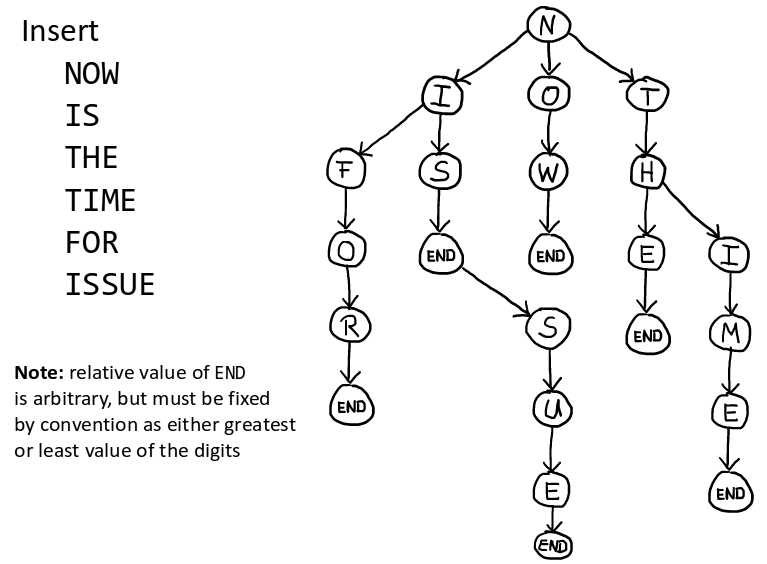
\includegraphics[width=0.625\linewidth]{img/tst} 
\end{figure}

\begin{itemize}
\item Works well for non-randomness in key structure (e.g. URLs). 
\item Search misses tend to be efficient. 
\item Good for suffix trees (index into shared text). 
\end{itemize}

\paragraph{Optimised TSTs}
\begin{itemize}
\item \emph{Wide head}: create table of $R$ TSTs. 
\item \emph{Compact tails}: store keys at leaves. 
\end{itemize}
\begin{figure}[H]
\centering{}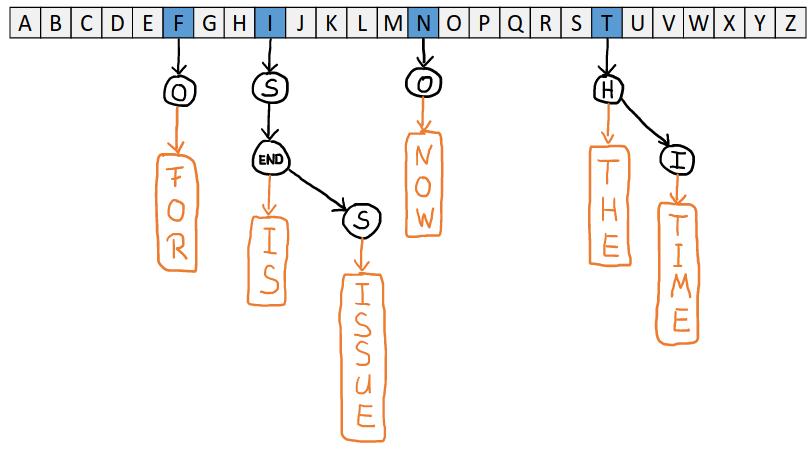
\includegraphics[width=0.7\linewidth]{img/opt-tst} 
\end{figure}



\section{Graph Algorithms}
\begin{itemize}
\item A graph $G=\left(V,E\right)$ can be represented as an adjacency-list
or matrix. 
\item A tree: 

\begin{itemize}
\item Has $V-1$ edges and no cycles. 
\item Has $V-1$ edges and is connected. 
\item Is connected, but removing any edge disconnects it. 
\item Is acyclic, but adding any edge creates a cycle. 
\item Exactly one simple path connects any pair of vertices. 
\end{itemize}
\end{itemize}

\paragraph{Breadth First Search}

Uses a queue, builds breadth-first trees, computes shortest paths.


\paragraph{Depth First Search}

Uses natural recursion, produces parenthesis structure.
\begin{itemize}
\item Edges classified as \emph{tree}, \emph{back} (point up the tree),
\emph{forward} (point down the tree) or \emph{cross}.
\end{itemize}

\paragraph{Parenthesis Theorem}

For any two vertices $u$ and $v$, one holds: 
\begin{enumerate}
\item $\left[u.d,u.f\right]$ and $\left[v.d,v.f\right]$ are completely
disjoint; neither $u$ nor $v$ is descendant of the other in the
depth-first forest. 
\item $\left[u.d,u.f\right]$ is entirely contained within $\left[v.d,v.f\right]$;
$u$ is a descendant of $v$ in a depth-first tree. 
\item $\left[u.d,u.f\right]$ and $\left[v.d,v.f\right]$ are completely
disjoint; $v$ is a descendant of $u$ in a depth-first tree. 
\end{enumerate}

\paragraph{Topological Sort}

Sort vertices by finish time of DFS.


\subsection{Spanning Tree}
\begin{enumerate}
\item A tree $T$. 
\item Includes all vertices $V$ of $G=\left(V,E\right)$. 
\item $T\subseteq E$. 
\end{enumerate}

\paragraph{Kruskal Algorithm}

Choose the edge of lowest weight as long as it doesn't create a cycle.


\subsection{Shortest Path}


\paragraph{Dijkstra Algorithm}

Choose the vertex with minimum distance, record predecessors. 
\begin{itemize}
\item Doesn't work for negative weights. 
\item Time complexity: $O\left(\left|V\right|\log\left|V\right|+\left|E\right|\right)$
using min-priority queue. 
\end{itemize}

\paragraph{Bellmann-Ford Algorithm}

Esentially Djisktra's algorithm applied $n$ times ($n$ is the number
of nodes). 
\begin{itemize}
\item Need to check for negative-weight cycles at end. 
\item Time complexity: $O\left(\left|V\right|\left|E\right|\right)$. 
\end{itemize}

\paragraph{Floyd-Warshall Algorithm}

\[
D_{ij}^{\left(k\right)}=\begin{cases}
w_{ij} & k=0\\
\min\left(D_{ij}^{\left(k-1\right)},D_{ik}^{\left(k-1\right)}+D_{kj}^{\left(k-1\right)}\right) & k\geq1
\end{cases}
\]

\begin{itemize}
\item Time complexity: $O\left(\left|V\right|^{3}\right)$. 
\end{itemize}

\paragraph{Johnson's Algorithm}

Better for sparse graphs. 
\begin{enumerate}
\item Add a new node $q$ connected to all other nodes with a zero-weight
edge. 
\item Use Bellman-Ford, starting from $q$ to get a minimum weight $h\left(v\right)$
for each node. 
\item Reweight the edges in the original graph \textemdash{} $w'\left(u,v\right)=w\left(u,v\right)+h\left(u\right)-h\left(v\right)$. 
\item Use Dijsktra algorithm. 
\end{enumerate}

\subsection{Maximum Flow}
\begin{itemize}
\item Remove anti-parallel edges using \emph{auxiliary vertices}. 
\item Deal with multiples sources and sinks by introducing \emph{supersources}
/ \emph{supersinks}. 
\end{itemize}

\paragraph{Constraints}
\begin{itemize}
\item \emph{Capacity constraint}: for all edges, flow must be less weight. 
\item \emph{Flow conservation}: for all non-source/sink vertices, flow in
= flow out. 
\end{itemize}

\paragraph{Ford-Fulkerson Method}

While there exists an \emph{augmenting path} $p$ in the \emph{residual
network}, augment flow $f$ along $p$.


\paragraph{Cuts}

If $f$ is the maximum flow $G$ $\left|f\right|=c\left(S,T\right)$
for some minimum cut $\left(S,T\right)$ in $G$. 
\end{document}
